%------------------------------------------------------------------------------
%	Setup
%------------------------------------------------------------------------------
\documentclass[journal, twocolumn]{IEEEtran}


\usepackage{graphicx}
\usepackage[breaklinks=true]{hyperref}
\usepackage{amsmath}
\usepackage{multirow}
\usepackage{amssymb}
\usepackage[noadjust]{cite}
\usepackage{filecontents}
\usepackage{tabularx,booktabs}
\usepackage{lipsum}

\usepackage{caption}
\usepackage{subcaption}
\captionsetup{font=footnotesize}

\usepackage{textcase}
\usepackage[tablename=TABLE]{caption}
\DeclareCaptionTextFormat{up}{\MakeTextUppercase{#1}}
\captionsetup[table]{
    labelsep=period,
    justification=centering,
    textformat=up,
}


% correct bad hyphenation here
\hyphenation{op-tical net-works semi-conduc-tor}


\begin{document}
%------------------------------------------------------------------------------
%	Title
%------------------------------------------------------------------------------
\title{An Automatic Face Attendance Checking System using Deep Facial Recognition Technique}


%------------------------------------------------------------------------------
%	Author
%------------------------------------------------------------------------------
\author{Thuy Nguyen-Chinh,
		Thien Do-Tieu,
		Sy Nguyen-Tan,
		Phuong Le-Van-Hoang,
		Qui Nguyen-Van,
		Phu Nguyen-Tan

\thanks{This work is a final project in the course "Artificial Intelligence in Control Engineering" (Aug-Dec 2018) guided by Dr. Cuong Pham-Viet (email: pvcuong@hcmut.edu.vn), Faculty of Electrical and Electronics Engineering, HoChiMinh city University of Technology.}
\thanks{Authors are senior students in the Faculty of Electrical and Electronics Engineering, University of Technology, HoChiMinh city Vietnam National University (e-mail: \{thuy.ng.ch, dotieuthien9997, tansyab1, hpcqt97, nvqui97, tanphu97.nguyen\}@gmail.com). The software is open source and can be found in \url{https://github.com/AntiAegis/Face-Attendance-System}.}
}


\maketitle


%------------------------------------------------------------------------------
%	Abstract
%------------------------------------------------------------------------------
\begin{abstract}
Nowadays, as computers are powerful enough for implementing complex algorithms, there are numerous applications that people utilize computers to run. In which, facial recognition is one of the most active fields of applications. In fact, computers can not only automatically identify who a person is, but also operate 24/7, which human beings cannot endure. This leads to the replacement of people by computers in some repetitive and real-time applications.

In this work, we apply the facial recognition into an attendance checking system that uses faces of registered people to check their attendance. This system has a GUI which allows easy user-to-system interaction. The core of the system is a deep facial recognition technique, which has four stages (e.g., removing motion-blur frames, detecting faces, removing non-frontal-view faces, and recognizing). Particularly, in the recognition phase, we consider this stage as an open-set facial recognition problem, so the system is able to detect people who have not registered in the database before. Also, we boost the performance of the system by utilizing hardware resources of users' computers. Although the system is designed to run with a low-resolution webcam, its performance is reasonably accurate on our private dataset.
\end{abstract}


\begin{IEEEkeywords}
Face Attendance Checking, Facial Recognition, Deep Learning
\end{IEEEkeywords}


\IEEEpeerreviewmaketitle


%------------------------------------------------------------------------------
%	Introduction
%------------------------------------------------------------------------------
\section{Introduction}
\label{introduction}

Face recognition systems are being applied widely in real life such as tracking, managing employees, finding information about celebrities, and so forth. There are many approaches to design a face recognition system, but such these systems are frequently affected by light, non-frontal faces, resolution of cameras, etc. Thus, each method has specific challenges. Overall, a face recognition has two main stages which are face detection and face recognition, yet we want to create constraints on blur-clean and frontal-view faces of users that leads our system to have four stages: blur detection, face detection, landmark detection, and face recognition.  


%------------------------------------------------------------------------------
\subsection{Face detection}
Before face recognition stage, we need to detect faces in a image and bound the high-level regions to eliminate effects, such as hair, background. The face detector proposed by Viola and Jones \cite{ref:detect-1} used Haar-Like features and AdaBoost algorithm to train cascaded classifiers, which achieve good performance with real-time efficiency. However, a few works \cite{ref:detect-2},\cite{ref:detect-3},\cite{ref:detect-4} show that Haar-Like feature may degrade considerably in real-world applications with larger visual variations of human faces even with more advanced features and more training images. Besides the cascade model, \cite{ref:detect-5},\cite{ref:detect-6},\cite{ref:detect-7} introduce deformable part models (DPM) for face detection and achieve remarkable performance. However, they need a high computational expense and may usually require expensive annotation in the training stage. With the rise of data-model, convolutional neural networks (CNN) achieve considerable accuracy in the number of computer vision tasks, especially face detection task. Li et al. \cite{ref:detect-8} use cascaded CNN for face detection, but it requires bounding box calibration from face detection with an extra computational expense and ignores the correlation between facial landmarks localization and bounding box regression. Face alignment also attracts extensive interests. Regression-based methods \cite{ref:detect-9},\cite{ref:detect-10},\cite{ref:detect-11} and template fitting methods \cite{ref:detect-7},\cite{ref:detect-12},\cite{ref:detect-13} are two popular approaches.

However, most of the available face detection and face alignment methods ignore the correlation between these two tasks. Though there exist several works attempt to jointly solve them, there are still limitations in these works. For example, Chen et al. \cite{ref:detect-14} jointly show alignment and detection with random forest using features of pixel value difference. But, the handcraft features used limits its performance. From those previous experiments, we choose a new approach which integrates these two tasks using unified cascaded CNN by multi-task learning called Multi-task Convolutional Network which is also face detector used in FaceNet model in section \ref{face-recognition}.


%------------------------------------------------------------------------------
\subsection{Landmark detection}
The locations of the facial landmark points around facial components (nose, eye centers, etc) capture facial deformations due to head movements and facial expressions, so we will control non-frontal faces for better accuracy. They are hence important for various facial analysis tasks. Many facial landmark detection algorithms have been developed to automatically detect those key points over the years. In this paper, we use Dlib library which is a powerfull opened source for face and facial landmark detection. We will discuss our implement in detail in section \ref{frontal-view-detection}.


%------------------------------------------------------------------------------
\subsection{Face recognition}
After face detection and alignment, those regions of a face are extracted to get feature vectors. Conventionally, one of the most popular features for face recognition is Gabor feature. Tudor Barbu \cite{ref:recog-1} used Gabor transform to extract features, and then applied K-Nearest Neighbour (K-NN) based on clustering features to predict identity of a face. This implementation achieved a quite impressed performance with an accuracy of 90\% on the Yale Face Database B \cite{ref:data-yaleB}. OpenCV \cite{ref:recog-2}, which is an open-source library focusing on Computer Vision algorithms, introduced a method called Local Binary Patterns (LBP) based on Haar-Like feature. In term of speed, LBP has a remarkably real-time efficiency, whereas it is not stable in term of accuracy. In particular, this method cannot face noise which is a reason why LBP and Haar-Like feature are rarely applied in practical systems. Because of limitations of conventional features, approaches exploiting deep learning have gradually developed instead. Yi Sun, Xiaogang Wang, and Xiaoou Tang \cite{ref:recog-3} built a deep model named Deep hidden IDentity (DeepID) which used Convolutional Neural Network (CNN) to extract face features. The advantage of this method was using a small dataset for training that was considerably relevant for applications which cannot collect a large dataset of users. Nevertheless, to reach a high accuracy, DeepID model became really complex with many neural network branches for each person. There were 10 patches of a face, which contain interesting information, chosen from each image, then they were scaled with three figures in RGB and gray channel. Totally, the model had 60 different networks to extract features for an image, then feedforwarded extracted features into a classifier using Joint Bayesian. DeepID achieved an excellent accuracy of 97.45\% on Labeled Faces in the Wild (LFW) \cite{ref:data-lfw}. In 2014, the authors of DeepID introduced DeepID2 \cite{ref:recog-4} which was an improved version of its predecessor. In the new version, interesting regions were built to eliminate useless patches which cannot provide high-level features. That work really helpfully affected the accuracy, specifically there was an increase in accuracy at 99.63\%. In 2015, Google Inc. \cite{ref:recog-5} exploited a deep CNN Inception \cite{ref:in-res} and a triplet loss function to form the FaceNet model, which was to extract features. Their outstanding point was using a hard triplet loss to separate features for each person, so FaceNet feature is robust in both face verification and face recognition. The accuracy of 99.63\% on LFW and 95.12\% on Youtube Faces DB \cite{ref:data-youtube} were high enough to represent the perfection of the model.


%------------------------------------------------------------------------------
%	Proposed system
%------------------------------------------------------------------------------
\medskip
\section{Proposed system}
\label{proposed-system}

In this paper, we apply deep facial recognition techniques to the problem of face attendance checking. A system is built in order to manage appearances of students in a class, which is revealed in Fig. \ref{fig:system}. Normally, a facial recognition system is organized as a pipeline of typical stages such as face detection, landmark detection, and face recognition. However, to ensure input frames for underlying algorithms are high quality, we append an early filter (the Blur detection stage) that are able to discard blur frames, which are caught by motions of people in front of a webcam. Then, clean frames are passed through the Face detection block for counting the number of faces existing inside these frames. In our specific constraint, there is only one face per frame allowed to be processed, so frames that contain more than one faces are rejected. Afterward, the Landmark detection is to localize statistic-salient points in the face in order to verify whether the face is in the frontal view of the camera. This frontal-view check will help improve the accuracy of the face recognition algorithm. Finally, the Face recognition uses blur-clean, one-face, and frontal-view frames from previous stages to extract relevant features and then perform a classification task to indicate which category the input most likely belong to.

In addition, to leverage the ease of use, we design a friendly graphic user interface (GUI) so that people who want to use the system to manage (teachers) or check (students) attendance can interact with the application without any specialized knowledge. To make the system more robust, we carefully analyze the distribution outlier of features representing for registered accounts. Therefore, the algorithm has ability to detect people who have not registered in the application before, which is equivalent to the open-set problem in face recognition.

Our work is organized as follows. In section \ref{implementation}, stages of the proposed system are described clearly, including motion-blur detection, face detection, frontal-view detection, and face recognition. Then, section \ref{experimental-result} is for reporting some experimental results.


\begin{figure}
    \centering
    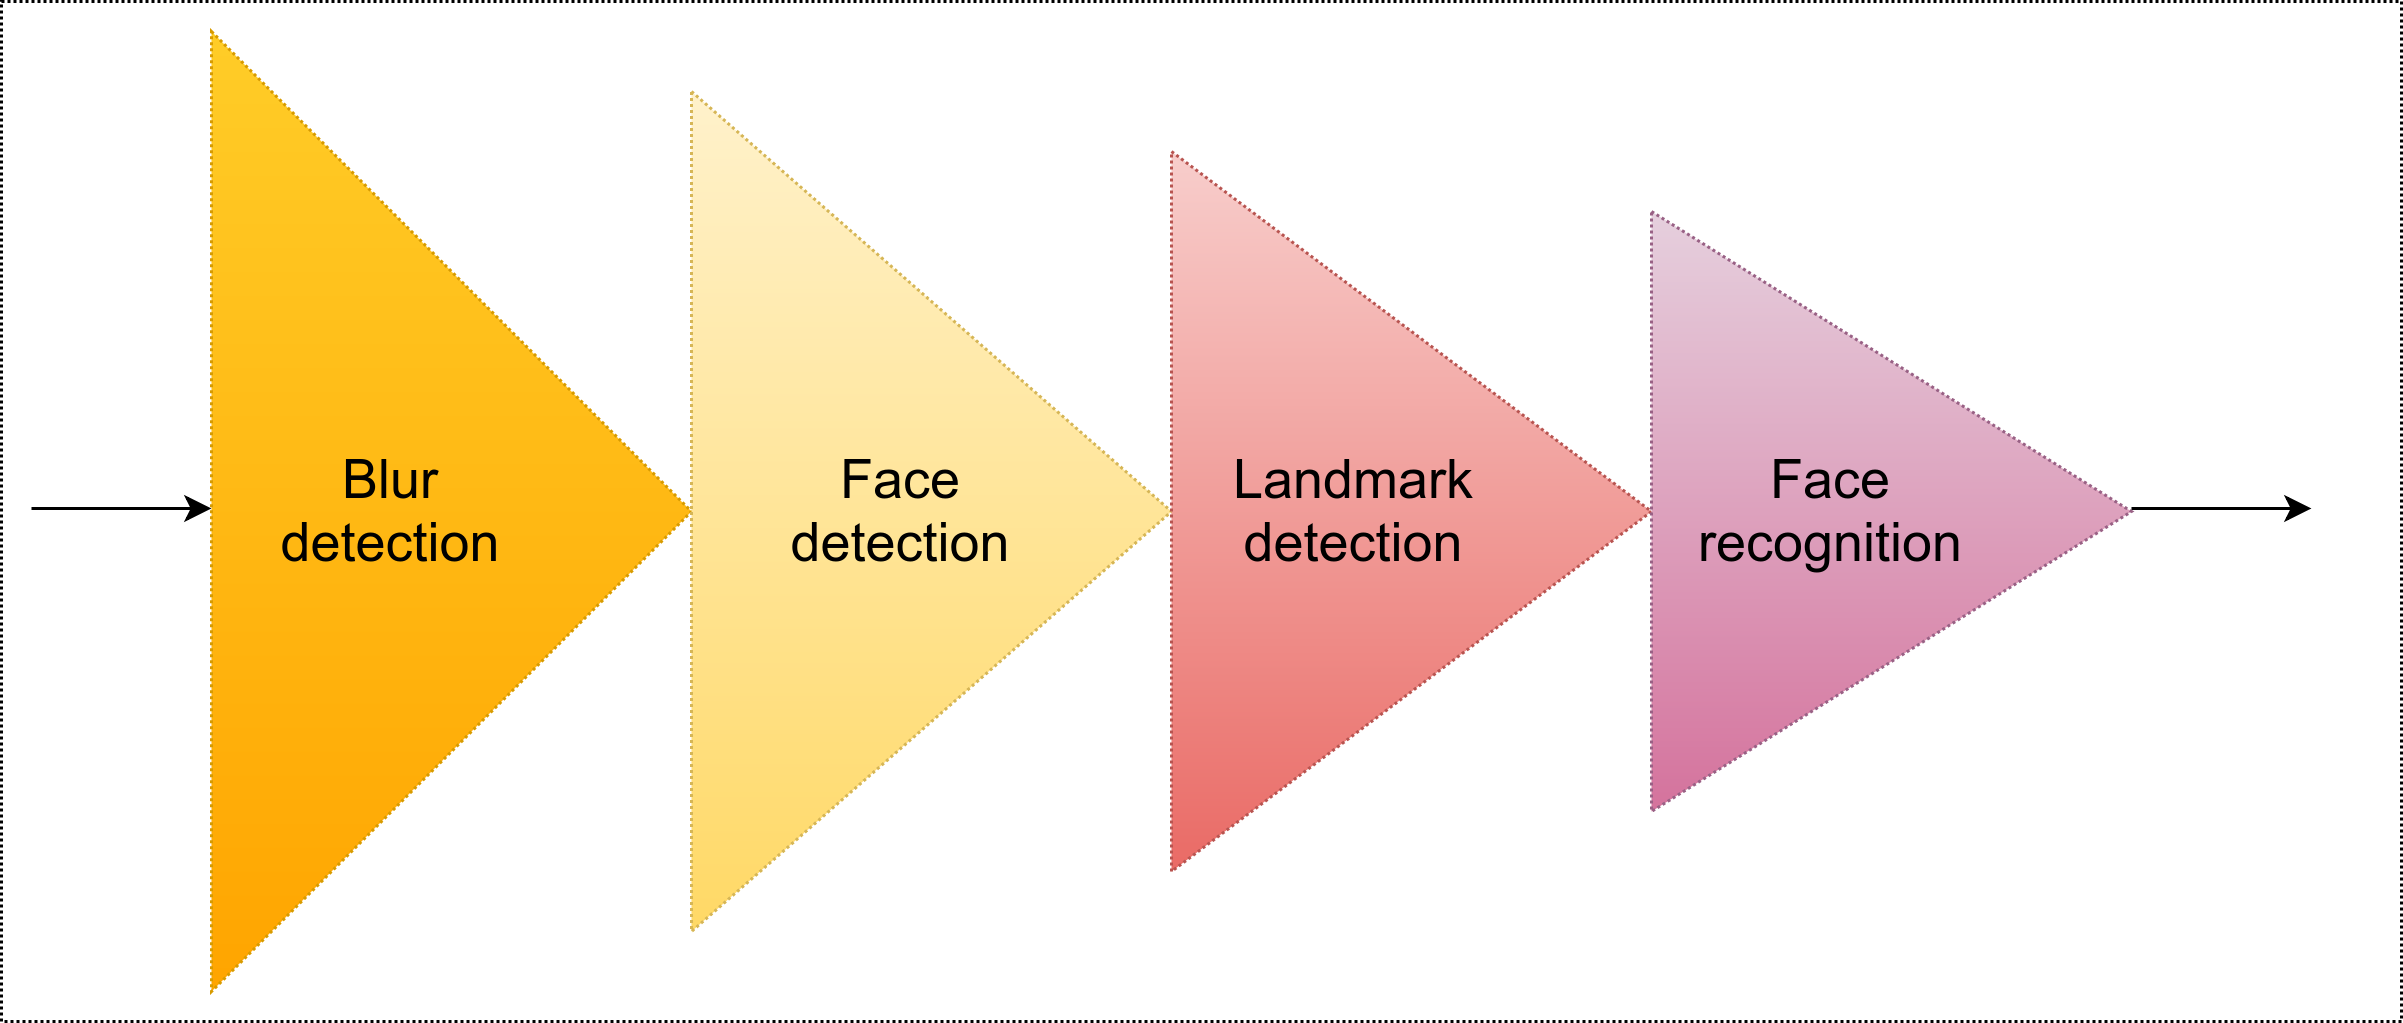
\includegraphics[width=\linewidth]{img/system-pipeline.png}
	\caption{The system pipeline. There are four stages, namely blur detection, face detection, landmark detection, and face recognition. These four blocks are in the descending order of size in the direction from input to output. This points out that our system is tougher to input frames from the camera when such frames passed through the system. Therefore, best frames are likely to be processed, which may improve the final recognition accuracy.}\label{fig:system}
\end{figure}


%------------------------------------------------------------------------------
%	Implementation
%------------------------------------------------------------------------------
\medskip
\section{Implementation}
\label{implementation}


%------------------------------------------------------------------------------
\subsection{Motion-blur detection}
\label{motion-blur-detection}

The first stage of this system is detecting blurred image and rejecting them out of next stage. We know that the blurred image means each pixel in the source image gets spread out and mixed into surrounding neighbour pixels. For our attendance checking system, the motion blur happens when an object (namely face or webcam) moves during the exposure. So as to detect whether an image is blurred, we use the 2D-FFT (2D-Fast Fourier Transform) method.

 We will review about Fourier Transform of Images. To compute the Fourier transform of an image, you need to:
\begin{itemize}
\item Compute DFT of each row, in place.
\item Compute DFT of each column, in place.
\end{itemize}  

When a signal is discrete and periodic, we use the discrete Fourier transform, or DFT.
Suppose our signal is $a_n$ for $n=0 \ldots N-1$,
and $a_n=a_{n+jN}$ for all $n$ and $j$.
The spectrum of $a$ is:
\begin{equation}
A_k = \sum_{n=0}^{N-1} W_N^{kn} a_n
\label{dft.eq}
\end{equation}
where
$$
W_N = e^{-i {2 \pi \over N}}
$$
and $W_N^k$ for $k=0 \ldots N-1$ are called the {\it Nth roots of unity}.
The sequence $A_k$ is the discrete Fourier transform of the sequence $a_n$.
Each is a sequence of $N$ complex numbers.

The FFT is a fast algorithm for computing the DFT.
If we take the 2-point DFT and 4-point DFT and generalize them
to 8-point, 16-point, ..., $2^n$-point (n is an integer), we get the FFT algorithm.

There are several ways to write an FFT. For instance, let $m$ be an integer and let $N=2^m$.
Suppose that $x=[x_0,\ldots,x_{N-1}]$ is an $N$ dimensional complex vector.
Let $\omega=\exp({-2\pi i\over N})$.  Then the DFT, $c= F_N(x)$ is given by
\begin{equation}
c_k={1\over N}\sum_{j=0}^{j=N-1}x_j\omega^{jk}.
\end{equation}
Let $n=N/2$, let $u$ and $v$ be $n$ dimensional vectors defined by 
\begin{align}
u_j&=x_j+x_{j+n},\ j=0,\ldots,n-1\\
v_j&=(x_j-x_{j+n})\omega ^j,\ j=0,\ldots,n-1.
\end{align}
Then 
\begin{align}
c_{2j}={1\over 2}(F_n(u))_j,\ j=0,\ldots,n-1\\
c_{2j+1}={1\over 2}(F_n(v))_j,\ j=0,\ldots,n-1.
\end{align}

To compute the DFT of an $N$-point sequence using equation (\ref{dft.eq})
would take $(N^2)$ multiplies and adds.
The FFT algorithm computes the DFT using $(N \log N)$ multiplies and adds.

Practical issues:
We translate the picture so that pixel (0,0), which now contains frequency $(\omega_x,\omega_y)=(0,0)$, moves to the center of the image. Then, we display pixel values proportional to
log(magnitude) of each complex number. For color images, do the above to each of the three channels
(R, G, and B) independently.

Apply to our system, firstly, we calculate FFT of image. Secondly, we will compute mean amplitude spectrum value of entire pixel in image and. Finally, the result of this operation is compared to an optimal threshold which distinguishes blurred and non-blurred image as accurate as possible. The image is called non-blurred if and only if its average value greater than the threshold value, and vice versa. After that, non-blurred images are applied to face detection stage of system.


%------------------------------------------------------------------------------
\subsection{Face detection}
\label{face-detection}

In this paper, we have used Histogram of Oriented Gradients method for extracting features of the face and Linear Support Vector Machine (SVM) method for face detections.\\
The implementation of this method using sliding window technique with the different sizes of the windows. Using the sliding window technique we could complete the calculation of HOG features, applied to detect and differentiate the face and the false face recognition using the SVM technique.\\
All of the pre-processing steps are automatically implemented before using Dlib library with the input of being given facial images and the output of localization the identified faces.\\


%------------------------------------------------------------------------------
\subsection{Frontal-view detection}
\label{frontal-view-detection}

To check whether the shape of the faces has to be frontal, we implement these 3 following steps:
\begin{enumerate}[Step 1.]
	\item Focusing on the center of the image. Only accept these faces that locate in the most central of the images. $((120-360), (90,360))$
	\item Identify the skew of the image: calculate the coordinate of these eyes and the angle deviation between two eyes in the horizontal direction. If the angle deviation is larger than 10 degree, the image will be ignored.
	\item Identify the rotation of the image: choose the point which is the midpoint of the right and the left eye. If the nose which is deviated from the selected point is greater than 10 pixels in the horizontal direction, the image is ignored.
\end{enumerate}
These steps are implemented based on 5-point facial landmark technique with Dlib library instead of 68-point facial landmark in order to improve performance. If the image satisfies the condition, it will be accepted.


%------------------------------------------------------------------------------
\subsection{Face recognition}
\label{face-recognition}
\begin{figure}
    \centering
    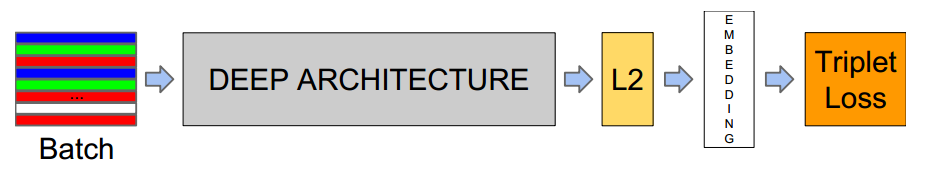
\includegraphics[width=1\linewidth]{img/pipeline.png}
	\caption{Model structure. Our network consists of a batch input layer and a deep CNN 
followed by L2 normalization, which results in the face embedding. This is followed by the triplet loss during training.}\label{fig:pipeline}
\end{figure}

In this stage, faces in raw images are detected and aligned by Multi-task CNN, we use convenient pre-trained FaceNet model to extract feature (in Figure \ref{fig:pipeline}) and then feedforward it to a SVM classifier for regconition. 


%------------------------------------------------------------------------------
\subsubsection{Multi-task Convolution Network}
\begin{figure}
    \centering
    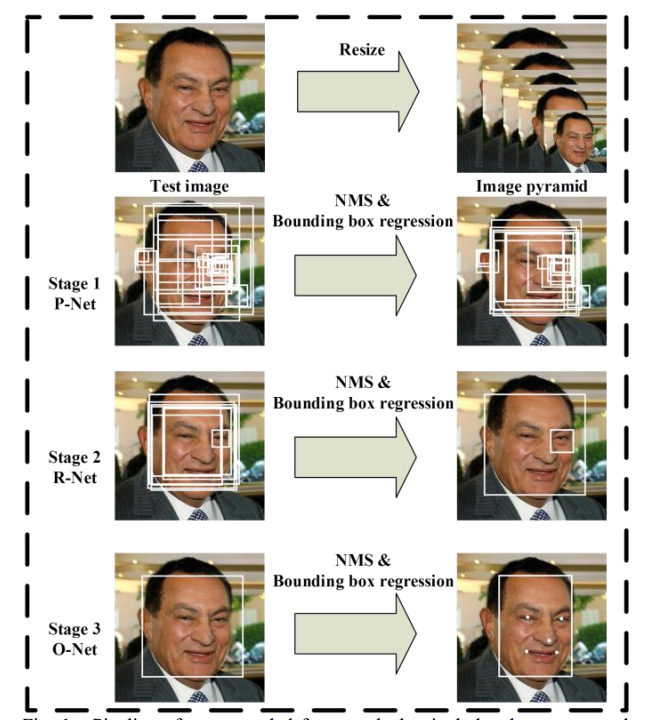
\includegraphics[width=1\linewidth]{img/mtcnn.png}
	\caption{Pipeline of our cascaded framework that includes three-stage multi-task deep convolutional networks. Firstly, candidate windows are produced
through a fast Proposal Network (P-Net). After that, we refine these candidates
in the next stage through a Refinement Network (R-Net). In the third stage,
The Output Network (O-Net) produces final bounding box and facial landmarks position.}\label{fig:mtcnn}
\end{figure}

The overall pipeline Multi-task CNN is shown in Figure \ref{fig:mtcnn}. An image is  initially resized to different scales to build an image pyramid, which is the input of the following three-stage cascaded framework with CNN architectures in Figure \ref{fig:mtcnn-arch}:

\textbf{Stage 1}: A fully convolutional network is exploited, called Proposal Network (P-Net), to obtain the proposed windows and their bounding box regression vectors. Then using the estimated bounding box regression vectors to calibrate the candidates. After that, employing non-maximum suppression (NMS) to merge highly overlapped candidates.

For each candidate window, P-CNN predict the offset between it and the nearest ground truth (i.e.,the bounding boxes’ left top, height, and width). The learning objective is formulated as a regression problem, and  the Euclidean loss is employed for each sample $x_i$:
\begin{align}
	L_i^{box} = \Vert y_i^{prediction} - y_i^{truth} \Vert _2^2
\end{align}
		
\textbf{Stage 2}: All candidates are fed to following CNN, called Refine Network (R-Net), which further rejects a large number of false candidates, performs calibration with bounding box regression, and NMS candidate merge.

\textbf{Stage 3}: his stage is similar to the second stage, but in this stage we aim to describe the face in more details. In particular, the network will output five facial landmarks’ positions.

Similar to the bounding box regression task, facial landmark detection is formulated as a regression problem: 

\begin{align}
	L_i^{landmark} = \Vert y_i^{prediction} - y_i^{truth} \Vert _2^2
\end{align}

\begin{figure}
    \centering
    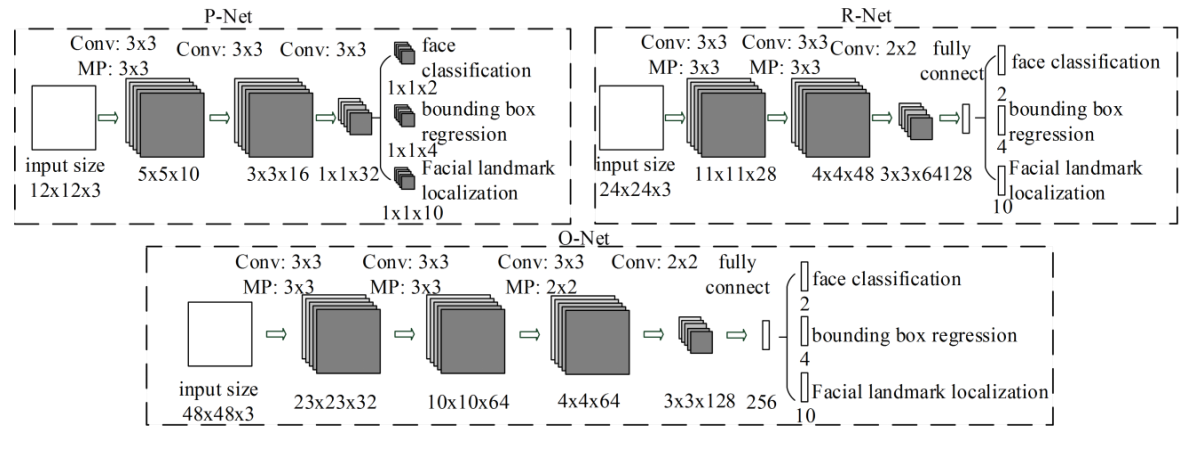
\includegraphics[width=1\linewidth]{img/mtcnn_arch.png}
	\caption{The architectures of P-Net, R-Net, and O-Net, where “MP” means max pooling and “Conv” means convolution. The step size in convolution and pooling
is 1 and 2, respectively}\label{fig:mtcnn-arch}
\end{figure}


%------------------------------------------------------------------------------
\subsubsection{FaceNet model} 
This model use Inception-ResNet v1 architecture \cite{ref:in-res} and triplet loss to extract feature. Inception-ResNet v1 (in Figure \ref{fig:inception-resnet}) is a very deep convolutional network which combine ResNet network and Inception network with a complex structure. This deep network affords to extract high-level feature for object recognition, and combination with triplet loss gets better and better. 

\begin{figure}
    \centering
    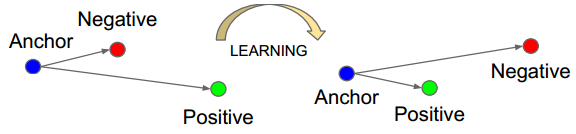
\includegraphics[width=1\linewidth]{img/triplet.png}
	\caption{The Triplet Loss minimizes the distance between an anchor and a positive, both of which have the same identity, and maximizes the distance between the anchor and a negative of a different identity.}
	\label{fig:triplet}
\end{figure}

The embedding is represented by $f(x) \in R^d$. It embeds an image $x$ into a $d$-dimensional Euclidean space. Here we want to ensure that an image $x_i^a$ (anchor) of a specific person is closer to all other images $x_i^p$ (positive) of the same person than it is to any image $x_i^n$ (negative) of any other person. This is visualized in Figure \ref{fig:triplet}. Thus we want, 
\begin{align}
	\Vert f(x_i^a) - f(x_i^p) \Vert_2^2 + \alpha < \Vert f(x_i^a) - f(x_i^n) \Vert_2^2
\end{align}
where $\alpha$ is a margin that is enforced between positive and negative pairs. The loss that is being minimized is then: 
\begin{align}
	L = \sum_i^N(\Vert f(x_i^a) - f(x_i^p) \Vert_2^2  - \Vert f(x_i^a) - f(x_i^n) \Vert_2^2 + \alpha)
\end{align}
In this implement, FaceNet model is trained on VGGFace2 dataset which over 9000 identities and over 3.3 million faces. VGGFace2 is a large-scale face recognition dataset from Google Image Search and have large variations in pose, age, illumination, ethnicity and profession. Therefore, embeddings is specifical for each person.


%------------------------------------------------------------------------------
\subsubsection{Training} 
To apply Multi-task model and FaceNet model into Face Attandence system, we feedforward raw images of students into Multi-task CNN to get face patches, then extract feature of each patch with 512 dimension vector by pre-trained FaceNet model \cite{ref:facenet}. After that, we split dataset of students into 3 subsets: training, validating and testing. Each person in training, validating, testing subset contains 30 images, 10 images and 30 images respectively. We decide to collect only 30 images for training subset, because we want to reduce time of training and time for collecting images. Especially, we also choose 4069 people who have only 1 image in LFW dataset for testing subset, because we want to evaluate the final accuracy of the whole algorithm. Next, we use SVM classifier with linear kernel to train on trainning subset and validate on validating subset. The formula of linear kernel:
\begin{align}
	probability = AX + b = W^TX^{bar} 
\end{align}
where $W$ is weight matrix, $X^{bar}=[1,x_1,x_2,...x_n]$. To solve multi-class classification problem, loss funtion of multi-class SVM is different from binary SVM. The output of trained-classifier is probability vector whose each element represent ability of an identity who anchor belong to. We assume $x_i$ is embedding $i^{th}$, $z_i$ is probability score of true label of $x_i$, $z_j$ ($j\ne i$) is probability scores of other classes of $x_i$ and $\Delta$ is safe distance to ensure $z_j$ is not much close with $z_i$. Loss value of $x_i$ with m classes is defined:
\begin{align}
	loss = \sum_{j=1}^m(max(0,z_j-(z_i-\Delta))
\end{align}
In dataset which has $n$ embeddings, total loss value is:
\begin{align}
	loss^{total} = \sum_{i=1}^n\sum_{j=1}^m(max(0,z_j-(z_i-\Delta))
\end{align}
This loss function will make $z_i$ is maximum. Thus, anchor is determined by choose which identity has maximum probability, that suffer from mistakes when faces of strangers appear. To solve open-set problem, we combine both two subsets: training and validating to training threshold. This threshold helps us to eliminate "unknow" people, additionally ensure that the result of system achieves higher accuracy.
\begin{figure}
    \centering
    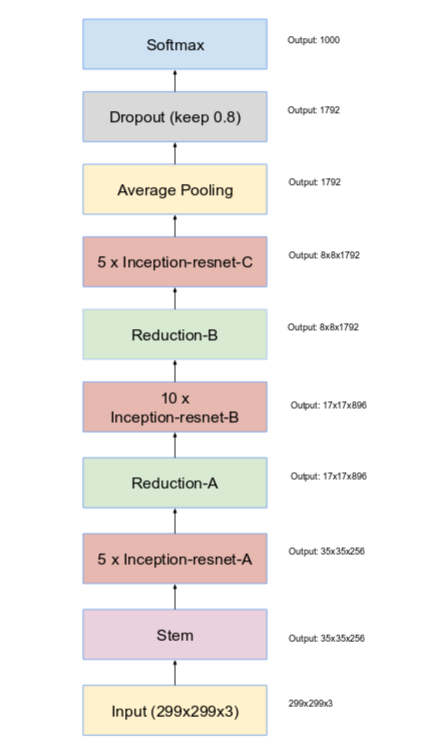
\includegraphics[width=0.7\linewidth]{img/in_res_v1.png}
	\caption{Schema for Inception-ResNet-v1 and Inception-ResNet-v2 networks. This schema applies to both networks but the underlying components differ.}
	\label{fig:inception-resnet}
\end{figure}


%------------------------------------------------------------------------------
\subsection{Graphic User Interface}
\label{gui}

The sections that follow describe how to create GUIs with PyQt5. This includes laying out the components, programming them to do specific things in response to user actions, and saving and launching the GUI; in other words, the mechanics of creating GUIs.

PyQt5 implements GUIs as figure windows containing various styles of uicontrol objects. You must program each object to perform the intended action when activated by the user of the GUI. In addition, you must be able to save graphical user interface development environment.

\textbf{GUI Development Environment}

The process of implementing a GUI involves two basic tasks:
\begin{itemize}
	\item Laying out the GUI components 
	\item Programming the GUI components
\end{itemize}
GUIDE primarily is a set of layout tools. However, you must create a PY-file that contains code to handle the initialization and launching of the GUI. This PY-file provides a framework for the implementation of the callbacks - the functions that execute and launch your GUI. 

\textbf{The Implementation of A GUI}

\textit{Laying out the GUI components}

While it is possible to write an PY-file that contains all the commands to lay out a GUI, it is easier to use GUIDE to lay out the components interactively and to generate one file that save the GUI:

UI-file -contains a complete description of the GUI figure and all of its children (uicontrols and axes), as well as the values of all object properties.

\textit{Programming the GUI components} 

Once you have the UI-file, you will use PyQt5 to extract the UI-file to PY-file to execute the program.PY-file -contains the functions that launch and control the GUI and the callbacks, which are defined as sub functions. This PY-file is referred to as the application PY-file in this documentation. Note that the application PY-file does not contain the code that lays out the uicontrols; this information is saved in the UI-file. The following diagram illustrates the parts of a GUI implementation.

\begin{figure}[!h]
	\centering
	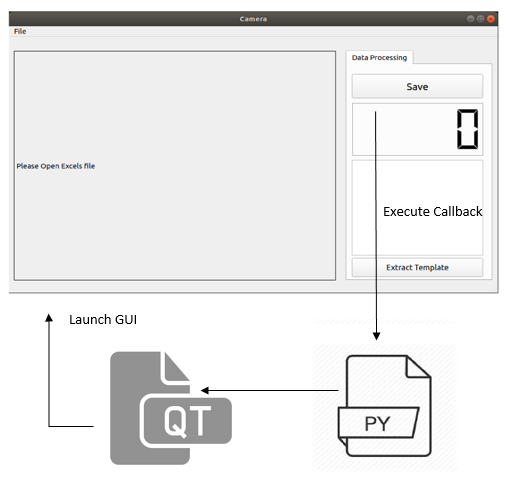
\includegraphics[width=0.8\linewidth]{img/gui.png}
	\caption{Parts of GUI Implementation}\label{fig:gui}
\end{figure}

The GUI are available from the QtDesigner shown in the figure below. The design is described briefly below. Subsequent sections show you how to use them.

\begin{figure}[!h]
	\centering
	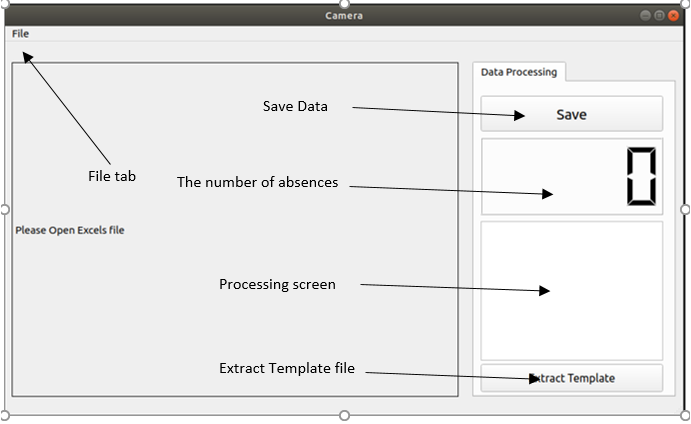
\includegraphics[width=0.8\linewidth]{img/user_guide.png}
	\caption{GUI layout}\label{fig:user_guide}
\end{figure}

\begin{table}[!h]
	\centering
	\begin{tabular}{|c|l|}
		\hline
		\textbf{uicontrols}                                                  & \multicolumn{1}{c|}{\textbf{function}}                                                                                                                                                                                                                                                                                                                                        \\ \hline
		\textbf{\begin{tabular}[c]{@{}c@{}}Open File\\  Option\end{tabular}} & \begin{tabular}[c]{@{}l@{}}We use this option to open the existing file\\  “Open” option appears and you can choose \\ to open the file.\end{tabular}                                                                                                                                                                                                                         \\ \hline
		\textbf{Start Camera}                                                & Open camera to start checking process                                                                                                                                                                                                                                                                                                                                         \\ \hline
		\textbf{Stop Camera}                                                 & Stop camera                                                                                                                                                                                                                                                                                                                                                                   \\ \hline
		\textbf{Exit}                                                        & \begin{tabular}[c]{@{}l@{}}We use this option to close the program. \\ we can follow the steps: \\ –Click on File tab \textgreater{}Exit, active file will be\\  closed. When we close the file, we get the\\  confirmation message to save the file or \\ not or cancel the command.\end{tabular}                                                                            \\ \hline
		\textbf{Save}                                                        & \begin{tabular}[c]{@{}l@{}}Store completely-checked student IDs on the\\ document. Once program exits, this process\\ will be automatically started so that you\\  won’t lose your work that has been\\  completed if there is a power interruption\\  or other system malfunction, the first time \\ you Save, it will take you to the\\  Save File dialog box.\end{tabular} \\ \hline
		\textbf{Extract Template}                                            & \begin{tabular}[c]{@{}l@{}}We use this option to export the template \\ in XLSX document. To Extract the file, \\ we can follow the steps:\\ – Click Extract Template . And then we can\\  export it as per our requirement.\end{tabular}                                                                                                                                     \\ \hline
	\end{tabular}
\caption{User Guide}\label{tab:user_guide}
\end{table}


%------------------------------------------------------------------------------
\subsection{Attendance management}
\label{attendance-management}

This is the final phase of Face Attendance Checking System.
It was designated to mark the presence of one resulted from
our algorithm in a file of excel format, namely xlsx extension.
To be used by the system, the excel file must meet
a stringent format made up of essential contents and be
generated by the GUI. 

Fig. \ref{fig:form-new} depicts a new standard empty
excel table generated by our GUI. After obtaining a new file, we should fill in the table with the desired data (Fig. \ref{fig:form-data}). The most special things in this table are column ID and Total. 
ID is considered a primary key because the algorithm will mark the presence of a specific person via his ID. 
To help the host in easy attendance management, we designed the column Total with a view to showing the number of absences in all.

Fig. \ref{fig:form-checked} depicts an excel file's content after a checking progress finished. 
The GUI will automatically insert the only one new day column between Group and Total ones and in the tail of previous checked day. 
Letter 1 will be marked as presence in a cell of this column accordant to an ID. 
After attendance checking process is completed, the Total column will display the number of absences of previous days and the current one. Smartly can it display as we specially assigned a size-dynamic sum function to each cell of this column.


\begin{figure}
    \centering
    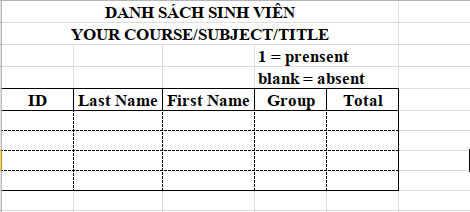
\includegraphics[width=0.8\linewidth]{img/form-new.png}
	\caption{New standard excel form}\label{fig:form-new}
\end{figure}

\begin{figure}
    \centering
    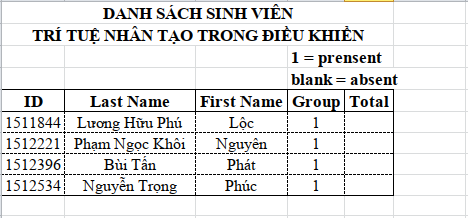
\includegraphics[width=0.8\linewidth]{img/form-data.png}
	\caption{Excel form contain pre-inputed data}\label{fig:form-data}
\end{figure}

\begin{figure}
    \centering
    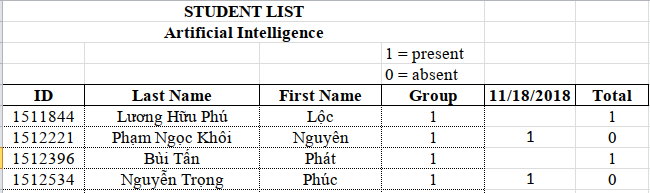
\includegraphics[width=0.8\linewidth]{img/form-checked.png}
	\caption{Form is under checking}\label{fig:form-checked}
\end{figure}


%------------------------------------------------------------------------------
%	Result
%------------------------------------------------------------------------------
\medskip
\section{Experimental result}
\label{experimental-result}

In this section, we first evaluate the effectiveness of the features extracted from FaceNet. Then, we compare our system in different contexts such as background, illumination, and resolution of camera, before examining the computational efficiency of our system.


%------------------------------------------------------------------------------
\subsection{Embeddings} 

\begin{figure}
  \centering
  
  \begin{subfigure}[b]{\linewidth}
	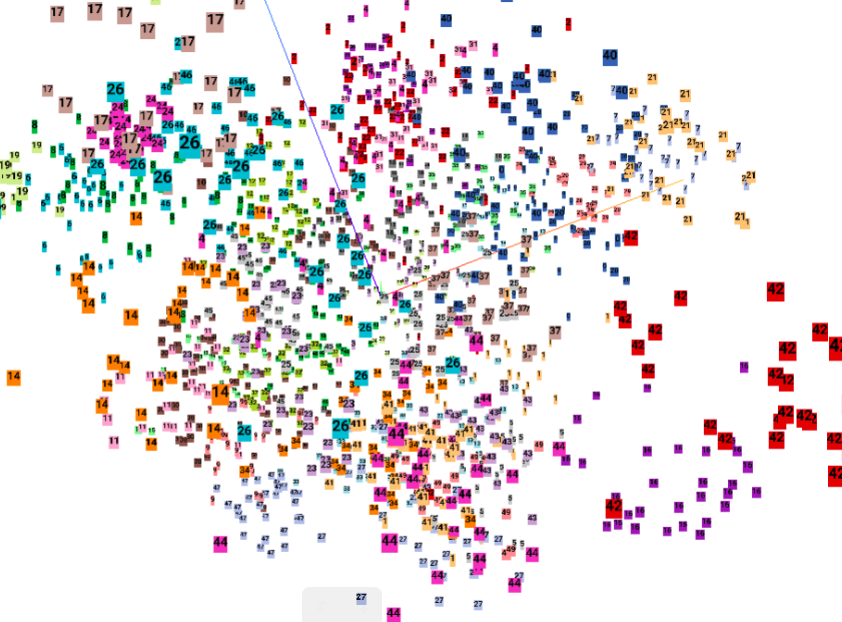
\includegraphics[width=\linewidth]{img/pca3.png}
    \caption{Visualization using PCA.}
    \label{fig:pca}
  \end{subfigure}
  
  \hspace{3mm}
  
  \begin{subfigure}[b]{\linewidth}
	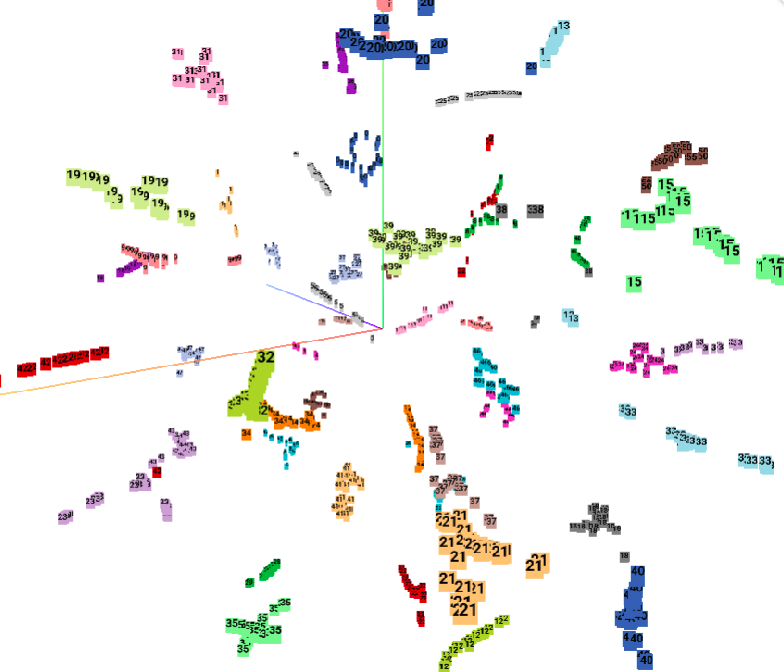
\includegraphics[width=\linewidth]{img/t-sne.png}
    \caption{Visualization using t-SNE.}
    \label{fig:t-sne}
  \end{subfigure}
  
  \caption{128-dimensional embeddings of the training set are projected to the 3D space using PCA (a) and t-SNE (b) techniques. In general, although samples of different classes are not totally separated, the PCA method partly reveals the separation of classes. Meanwhile, the t-SNE method provides a better view of classes as distinguished clusters. Best viewed in color.} 
  \label{fig:visualization}
\end{figure}


As mentioned above, features representing for faces play a crucial role in a robust face recognition algorithm. A good kind of feature is a way of representing input data so that data points belonging to a same category are close together, whereas, those ones which are different from their categories need to be as far as possible. Therefore, before training the model, we start evaluating how separate samples of different classes stand in a vector space.

In this work, we utilize the pre-trained model FaceNet because of its spectacular demonstration over the recent period. Embedding or the feature vector of FaceNet has size of 128. Therefore, in a 128-dimensional space, embeddings of samples should form clusters, in which, a cluster is a set of samples in a same class. Nevertheless, the 128-dimensional space is beyond human's vision and awareness. Therefore, to have a prior look on these embeddings, we use visualization methods so that embeddings are converted into a new vector space, which human can understand.

Here we exploit the Principal Component Analysis (PCA) and t-SNE \cite{ref:t-sne} to complete this task. The two methods project embeddings from the original size into the 3D space. The result of projection is depicted in Fig. \ref{fig:visualization}. In particular, PCA visualization selects eigenvectors corresponding to the highest eigenvalues as basics for constructing a new 3D space. Thus, its result in Fig. \ref{fig:pca}, although, illustrates that data points are slightly separated between distinct classes, this separation is still not clear. The reason is non-selected (residual) eigenvectors still convey a significant amount of information, so by removing them, there is more spatial information is lost. Meanwhile, in Fig. \ref{fig:t-sne}, the separation illustration is picturesque. Inter-class samples are closed while intra-class samples are far from each other. This is because the t-SNE method includes a clustering stage, so embeddings totally belong to their classes. If embeddings of FaceNet do not contain high-level specification, dimension reduction algorithms cannot show or cluster embeddings properly. Consequently, embeddings of the pre-trained FaceNet are sufficient for us to train a classifier for indicating the most likely class that an input belongs to, so we do not conduct a further finetuning stage to adapt the pre-trained FaceNet model in order to be compatible to our dataset.


%------------------------------------------------------------------------------
\subsection{Training}
<<<<<<< HEAD
Training data is carefully collected with different views from $-70^\circ$ to $70^\circ$. This work can improve accuracy in pratical system ,because it is difficult for users to keep their faces in a correct position. Training data include 52 identities and 1560 images totally. The training accuracy and the validating accuracy of SVM classifier is 100\% and 99.22\% respectively (in Figure \ref{fig:acc}). In Figure \ref{fig:loss}, the convergence of loss can indicate that this model achieves a good performance without overfitting. 
=======
Training data is carefully selected with different views from $-70^\circ$ to $70^\circ$. This work can improve accuracy in practical system, because it is difficult for users to keep their faces in a correct position. Therefore, by choosing faces with view variations, the model learns to generalize from training data. The training set includes 52 identities (people), in which, each identity consists of 30 images with various poses. This results in the training set of 1560 images totally. The training accuracy and validating accuracy of SVM classifier is 100\% and 99.22\% respectively (in Figure \ref{fig:acc}). In Figure \ref{fig:loss}, the convergence of loss can indicate that this model achieves a good performance without overfitting.


>>>>>>> 43009f34fee70080711d3256220dccf0d99f6d6d
\begin{figure}
    \centering
    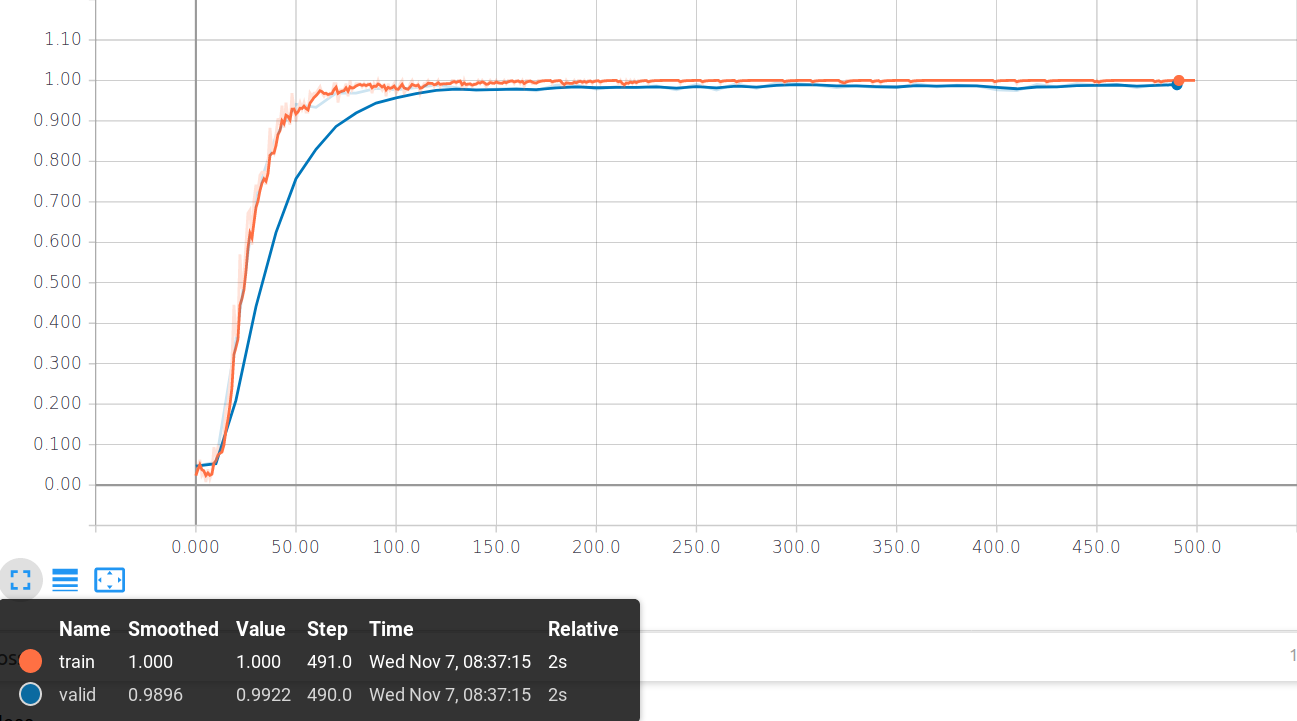
\includegraphics[width=1\linewidth]{img/acc.png}
	\caption{Accuracy in training and validating stage.}
	\label{fig:acc}
\end{figure}


\begin{figure}
    \centering
    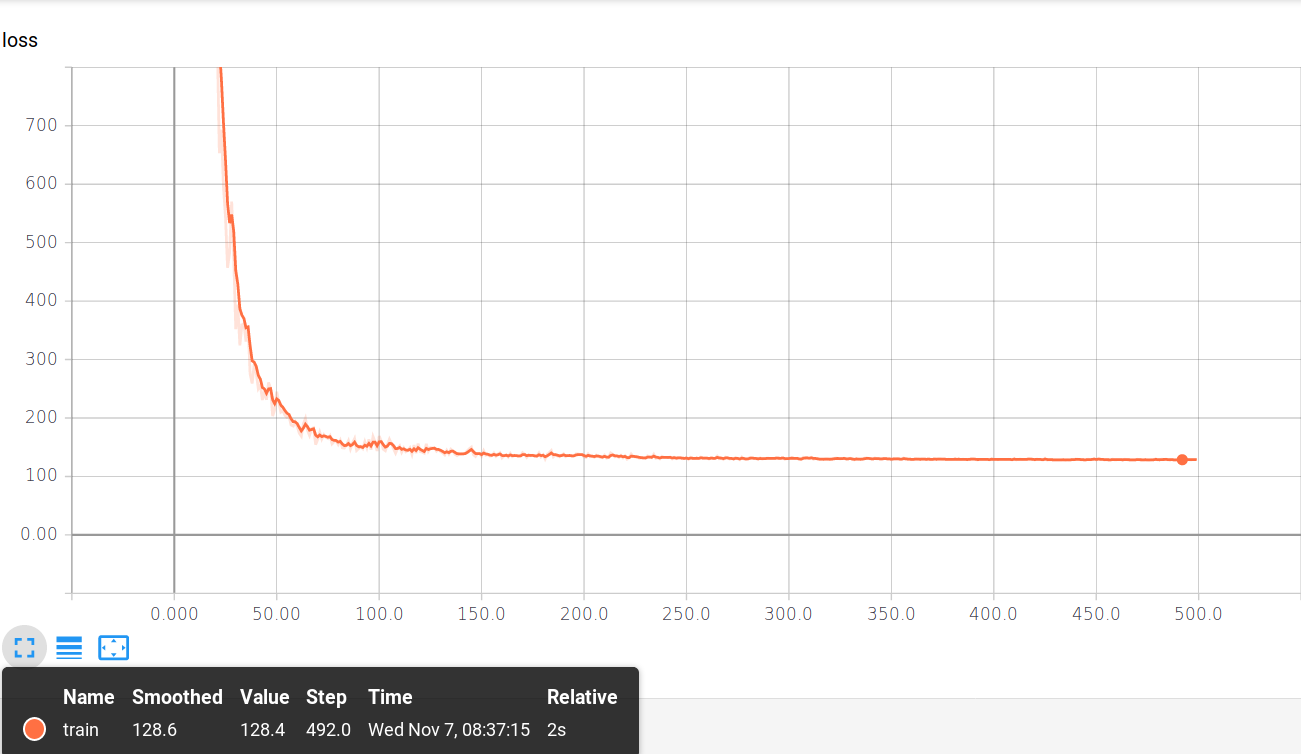
\includegraphics[width=1\linewidth]{img/loss.png}
	\caption{Loss value of SVM with linear kernel.}
	\label{fig:loss}
\end{figure}
<<<<<<< HEAD
We try to implement multi-class SVM by using API of sklearn library, the training accuracy of 100\% and the validating accuracy of 99.36\% are slightly the same in comparison with the above SVM model. After training classifier, we train to get the best threshold to determine "unknown" people. We divide threshold in range $[0;1]$ and then select a maximum value which make model achieves the best accuracy. Particularly, the model ignores people who have the scores being lower than threshold, and we combine the training subset and the validating subset for training threshold. Our dataset of students is collected once a semester, so training threshold with only training subset cause overfitting and difficult recognizing for reality system. As a result, threshold for 52 identities is 0.18825 in Figure \ref{fig:thres}. Testing accuracy with threshold achieves 96.48\% on testing subset, which is shown in Table \ref{tab:summary}. In practical environment, we test on 32 identities, three are 29 identites recognized easily and 3 identities who are not recognized continuously. In Figure \ref{fig:compare}, the (a),(b) are training images and (c),(b) are testing images, the effect of different ilumination lead the probabilities of testing anchor are lower than threshold, so training data have to cover many real-life cases to create the best classifier.  
\begin{figure}
    \centering
    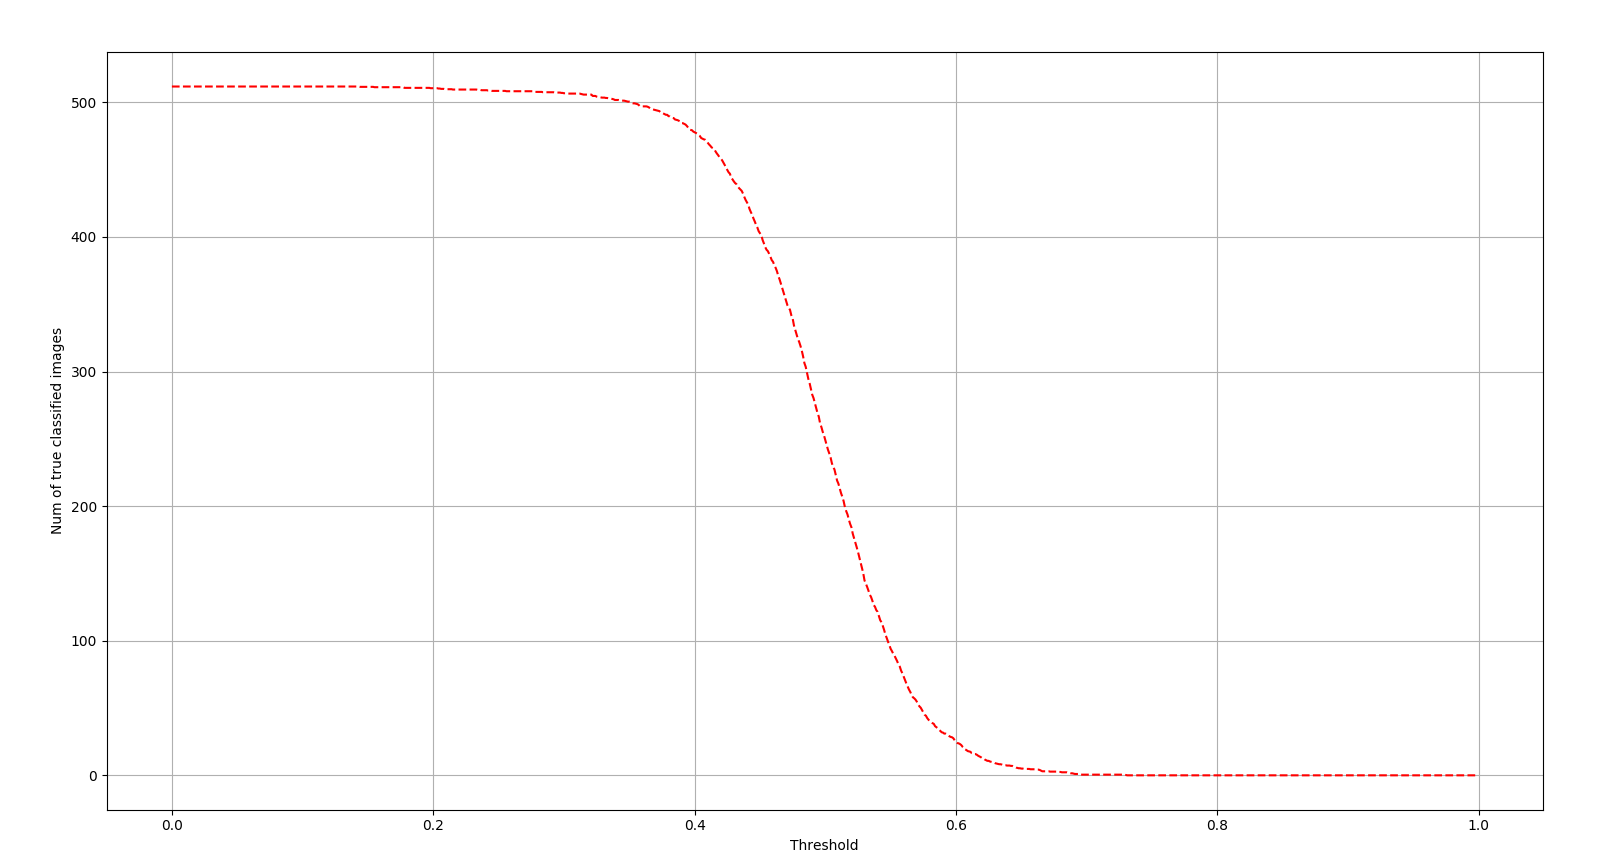
\includegraphics[width=1\linewidth]{img/thres.png}
	\caption{Training threshold stage, the final threshold is 0.18825}\label{fig:thres}
\end{figure}
=======


\begin{table}
\centering
	\caption{Dataset summary}
	\label{table:dataset}
		\begin{tabularx}{0.65\linewidth}{lcc}
		\toprule
		Dataset      &   Number of  &  Number of images  \\ 
		~            &  identities  &  per identity  \\
		\midrule
		Training     &   52  &  30  \\ 
		Validating   &   52  &  10  \\ 
		Testing      &   52  &  30  \\ 
		Unknown      &   xx  &  xx  \\ 
		\bottomrule
	\end{tabularx}
\end{table}


We try to implement multi-class SVM by using sklearn library and the accuracy is 99.36\%. After training classifier, we train to get the best threshold. We divide threshold in range $[0;1]$. As a result, threshold for 52 identities is 0.18825. Testing accuracy with threshold achieve 98.85\% on testing subset. In practical environment, we test on 32 identities, three are 29 identites recognized easily and 3 identities who are not recognized continuously. In Figure \ref{fig:compare}, the (a),(b) are training images and (c),(b) are testing images, the effect of different ilumination lead the probabilities of testing anchor are lower than threshold, so training data have to cover many real-life cases to create the best classifier.  
>>>>>>> 43009f34fee70080711d3256220dccf0d99f6d6d

\begin{figure}[h!]
  \centering
  \begin{subfigure}[b]{0.35\linewidth}
    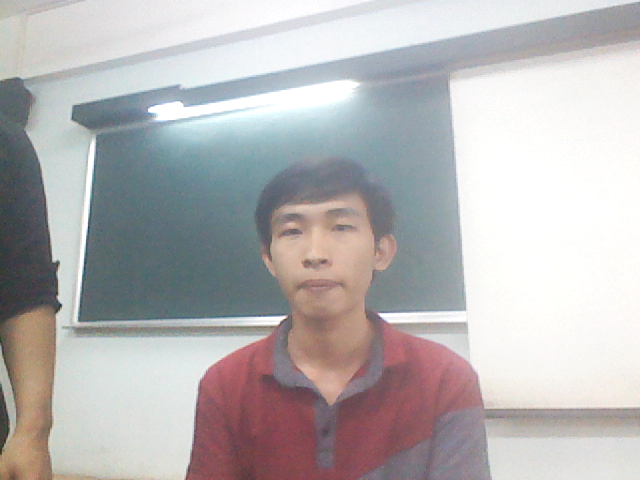
\includegraphics[width=\linewidth]{img/1.png}
    \caption{}
  \end{subfigure}
  \begin{subfigure}[b]{0.35\linewidth}
    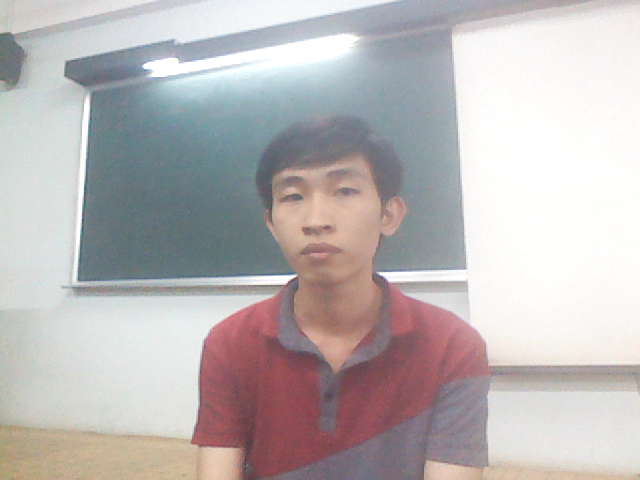
\includegraphics[width=\linewidth]{img/2.png}
    \caption{}
  \end{subfigure}
  \begin{subfigure}[b]{0.35\linewidth}
    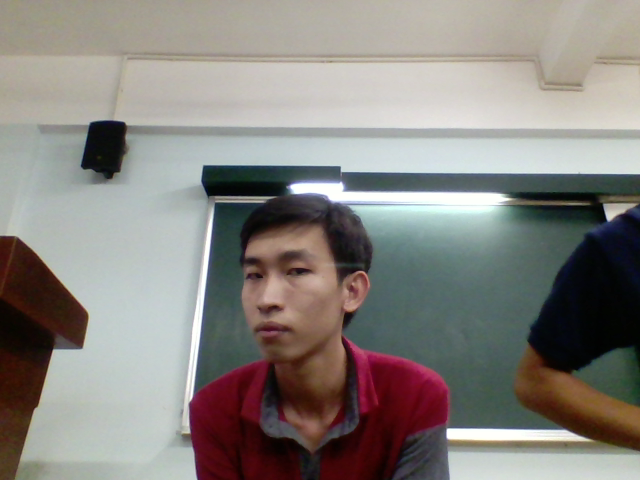
\includegraphics[width=\linewidth]{img/3.png}
    \caption{}
  \end{subfigure}
    \begin{subfigure}[b]{0.35\linewidth}
    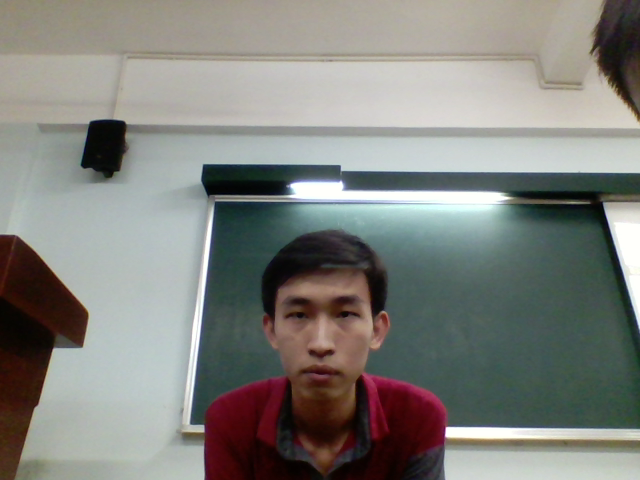
\includegraphics[width=\linewidth]{img/4.png}
    \caption{}
  \end{subfigure}
  \caption{Unrecognized identity, (a),(b) are training images, and (c),(d) are testing images in pratical condition.} 
  \label{fig:compare}
\end{figure}


\begin{table}[!h]
\centering
\caption{Summary}\label{tab:summary} 
\begin{tabular}{|c|c|c|c|c|} 
\hline
Stage & Training & Validating & Testing \\
\hline
Num of images & 1560 & 520 & 5109 \\ 
\hline
Num of identites & 52 & 52 & 4121 \\ 
\hline
Accuracy & 100\% & 99.36\% & 96.48\% \\
\hline
\end{tabular}
\end{table}


%------------------------------------------------------------------------------
%	Conclusion
%------------------------------------------------------------------------------
\medskip
\section{Conclusion}
\label{conclusion}

In this work, we applied the deep facial recognition techniques to solve the problem of face attendance checking. The system has a pipeline with four stages (e.g., motion-blur detection, face detection, landmark detection, and face recognition). Besides, the system is also integrated a friendly GUI, which allows users both teachers and students interact with it in an easy way. On our private dataset, the application performs accurately despite the low-resolution webcam on typical laptops. This demonstrates that our underlying algorithm is effective to deal with this poor-quality input problem.

In the future, we will target to widen our dataset so that the dataset can be asymptotic to real applications. In addition, more algorithms will be considered to improve the ability of the algorithm to discriminate feature distributions of output classes.


%------------------------------------------------------------------------------
%	Acknowledgment
%------------------------------------------------------------------------------
\section*{Acknowledgment}

The authors would like to acknowledge Dr. Cuong Pham-Viet for providing documents as well as promoting the chance for us to do this work. Also, the authors would like to thank volunteer students in the course EE3063 (Aug-Dec 2018, HoChiMinh city University of Technology), who donated data for us to conduct this work.


%------------------------------------------------------------------------------
% References
%------------------------------------------------------------------------------
\begin{thebibliography}{9}
%% Copy-Move-------------------------------------------------------------------
%%%% Key-point-based
\bibitem{ref:keypoint-1}
X. Pan and S. Lyu,
\textit{``Region duplication detection using image feature matching"},
IEEE Transactions on Information Forensics and Security,
vol. 5, no.4, ISSN: 1556-6013, pp. 857-867, 2010.
	
\bibitem{ref:keypoint-2}
I. Amerini, L. Ballan, R. Caldelli, A. Del Bimbo and G.Serra,
\textit{``A sift-based forensic method for copy–move attack detection and transformation recovery"},
IEEE Transactions on Information Forensics and Security,
vol. 6, no. 3, ISSN: 1556-6013, pp. 1099-1110, 2011.

\bibitem{ref:keypoint-3}
P. Kakar, N. Sudha,
\textit{``Exposing postprocessed copy-paste forgeries through transform-invariant feature"},
IEEE Transactions on Information Forensics and Security,
vol. 7, no. 3, ISSN: 1556-6013, pp. 1018-1028, June 2012.

%%%% Block-based
\bibitem{ref:block-1}
S.-J. Ryu, M.-J. Lee and H.-K. Lee,
\textit{``Detection of copy-rotate-move forgery using Zernike moments"},
Information Hiding Conference, Lecture Notes in Computer Science, vol. 6387, Springer,
Heidelberg-Berlin, 2010, ISBN: 978-3-642-16434-7.

\bibitem{ref:block-2}
H.-J. Lin, C.-W. Wang and Y.-T. Kao,
\textit{``Fast copy-move forgery detection"},
WSEAS Transactions on Signal Processing,
vol. 5, no. 5, ISSN: 0031-3203, pp. 188-1975, 2009.

\bibitem{ref:block-3}
V. Christlein, C. Riess, J. Jordan and E. Angelopoulou,
\textit{``An evaluation of popular copy-move forgery detection approaches"},
IEEE Transactions on Information Forensics and Security,
vol. 7, no. 6, ISSN: 1556-6013, pp. 1841-1854, 2012.

\bibitem{ref:block-4}
T. L.-Tien, T. H.-Kha, L. P.-C.-Hoan, A. T.-Hong, N. Dey, M. Luong,
\textit{``Combined Zernike Moment and Multiscale Analysis for Tamper Detection in Digital Images"},
Informatica (An International Journal of Computing and Informatics),
vol.41, no.1, ISSN: 0350-5596, March 2017.


%% JPEG format-----------------------------------------------------------------
\bibitem{ref:jpeg-dct-1}
Z. Lin, J. He, X. Tang, K. Tang,
\textit{``Fast, automatic and fine-grained tampered JPEG image detection via DCT coefficient analysis"},
Pattern Recognition, vol. 42, no. 11, ISSN: 0031-3203, pp. 2492-2501, January 2009.

\bibitem{ref:jpeg-dct-2}
W. Wang, J. Dong, T. Tan,
\textit{``Exploring DCT coefficient quantization effects for local tampering detection"},
IEEE Transactions on Information Forensics and Security,
vol. 9, no. 10, ISSN: 1556-6013, pp. 1653-1666, October 2014.

\bibitem{ref:jpeg-periodicity}
L. Chen, T. Hsu,
\textit{``Detecting recompression of JPEG images via periodicity analysis of compression artifacts for tampering detection"},
IEEE Transactions on Information Forensics and Security,
vol. 6, no. 2, ISSN: 1556-6013, pp. 396-406, June 2011.

\bibitem{ref:jpeg-improved}
L. Thing, Y. Chen, C. Cheh,
\textit{``An improved double compression detection method for JPEG image forensics"},
In IEEE International Symposium on Multimedia,
pages 290-297, December 2012, ISBN: 978-1-4673-4370-1.

\bibitem{ref:jpeg-ghosts}
F. Zach, C. Riess, and E. Angelopoulou,
\textit{``Automated image forgery detection through classification of JPEG ghosts"},
Pattern Recognition, 7476, pp. 185-194, January 2012.

\bibitem{ref:jpeg-block-grained}
T. Bianchi, A. Piva,
\textit{``Image forgery localization via block-grained analysis of JPEG artifacts"},
IEEE Transactions on Information Forensics and Security,
vol. 7, no. 3, ISSN: 1556-6013, pp. 1003-1017, June 2012.

\bibitem{ref:jpeg-inpainting}
C. Chang, C. Yu, C. Chang,
\textit{``A forgery detection algorithm for exemplar-based inpainting images using multi-region relation"},
Journal Image and Vision Computing,
vol. 31, no. 1, ISSN: 0262-8856, pp. 57-71, MA-USA, 2013.


%% Deep Learning approach------------------------------------------------------
\bibitem{ref:cnn-median}
J. Chen, X. Kang, Y. Liu and Z. J. Wang,
\textit{``Median Filtering Forensics Based on Convolutional Neural Networks"},
IEEE Signal Processing Letters,
vol. 22, no. 11, ISSN: 1070-9908, pp. 1849-1853, November 2015.

\bibitem{ref:cnn-universal}
B. Bayar, M. C. Stamm,
\textit{``A Deep Learning Approach to Universal Image Manipulation Detection Using a New Convolutional Layer"},
Proceedings of the 4th ACM Workshop on Information Hiding and Multimedia Security,
pp. 5-10, New York-USA, 2016, ISBN: 978-1-4503-4290-2.

\bibitem{ref:cnn-srm}
Rao Yuan, Ni Jiangqun,
\textit{``A deep learning approach to detection of splicing and copy-move forgeries in images"},
IEEE International Workshop on Information Forensics and Security (WIFS),
Abu Dhabi-United Arab Emirates, 2016, ISBN: 978-1-5090-1139-1.

\bibitem{ref:cnn-alex}
J.Ouyang, Y.Liu, M.Liao,
\textit{``Copy-Move Forgery Detection Based on Deep Learning"},
10th International Congress on Image and Signal Processing, BioMedical Engineering and Informatics,
Shanghai-China, 2017, ISBN: 978-1-5386-1938-4.

\bibitem{ref:dae}
Y. Zhang, J. Goh, L. Win, V. Thing,
\textit{``Image Region Forgery Detection: A Deep Learning Approach"},
Proceedings of the Singapore Cyber-Security Conference, Singapore, 2016, ISBN: 978-1-61499-616-3.


%% Database--------------------------------------------------------------------
\bibitem{ref:casia}
J. Dong and W. Wang,
\textit{``Casia tampering detection dataset"}, 2011.


%% Machine Learning------------------------------------------------------------
\bibitem{ref:alex-net}
A. Krizhevsky, I. Sutskever, G. Hinton,
\textit{``Imagenet classification with deep convolutional neural networks"},
NIPS'12 Proceedings of the 25th International Conference on Neural Information Processing Systems,
vol. 1, pp. 1097-1105, Nevada-USA, 2012, DOI: 10.1145/3065386.

\bibitem{ref:dropout}
N. Srivastava, 	G. Hinton, A. Krizhevsky, I. Sutskever, R. Salakhutdinov,
\textit{``Dropout: a simple way to prevent neural networks from overfitting"},
The Journal of Machine Learning Research,
vol. 15, no. 1, ISSN 1533-7928, pp. 1929-1958, January 2014.

\bibitem{ref:xavier}
Xavier Glorot, Yoshua Bengio,
\textit{``Understanding the difficulty of training deep feedforward neural networks"},
Proceedings of the 13rd International Conference on Artificial Intelligence and Statistics,
PMLR 9, pp. 249-256, Sardinia-Italy, \url{http://proceedings.mlr.press/v9/glorot10a/glorot10a.pdf}, 2010.

\bibitem{ref:relu}
V. Nair, E. Hinton,
\textit{``Rectified Linear Units Improve Restricted Boltzmann Machines"},
Proceedings of the 27th International Conference on Machine Learning,
pp. 807-814, Haifa-Israel, 2010, ISBN: 978-1-60558-907-7.

\bibitem{ref:leaky-relu-1}
B. Xu, N. Wang, T. Chen, M. Li,
\textit{``Empirical Evaluation of Rectified Activations in Convolutional Network"},
\url{https://arxiv.org/abs/1505.00853v2}, 2015.

\bibitem{ref:leaky-relu-2}
K. He, X. Zhang, S. Ren, J. Sun
\textit{``Delving Deep into Rectifiers: Surpassing Human-Level Performance on ImageNet Classification"},
\url{https://arxiv.org/abs/1502.01852v1}, 2015.

\bibitem{ref:adam}
P. Kingma, J. Ba,
\textit{``Adam: A Method for Stochastic Optimization"},
3rd International Conference for Learning Representations, San Diego-USA,
\url{https://arxiv.org/abs/1412.6980}, 2015.


%% Comparison------------------------------------------------------------------
\bibitem{ref:goh}
J. Goh and V. L. L. Thing,
\textit{``A hybrid evolutionary algorithm for feature and ensemble selection in image tampering detection"},
International Journal of Electronic Security and Digital Forensics,
vol. 7, no. 1, ISSN: 1751-911X, pp. 76-104, March 2015.

\bibitem{ref:he}
Z. He, W. Lu, W. Sun, J. Huang,
\textit{``Digital image splicing detection based on Markov features in DCT and DWT domain"},
Pattern Recognition, vol. 45, no. 12, ISSN: 0031-3203, pp. 4292-4299, 2012.


%% Appendix--------------------------------------------------------------------
\bibitem{ref:prove-wavelet}
A. Cohen, T. Tiplica, and A. Kobi,
\textit{``Design of experiments and statistical process control using wavelets analysis"},
Control Engineering Practice,
vol. 49, ISSN: 0967-0661, pp. 129-183, April 2016.


\end{thebibliography}

\end{document}
